%% bare_conf.tex
%% V1.3
%% 2007/01/11
%% by Michael Shell
%% See:
%% http://www.michaelshell.org/
%% for current contact information.
%%
%% This is a skeleton file demonstrating the use of IEEEtran.cls
%% (requires IEEEtran.cls version 1.7 or later) with an IEEE conference paper.
%%
%% Support sites:
%% http://www.michaelshell.org/tex/ieeetran/
%% http://www.ctan.org/tex-archive/macros/latex/contrib/IEEEtran/
%% and
%% http://www.ieee.org/

%%*************************************************************************
%% Legal Notice:
%% This code is offered as-is without any warranty either expressed or
%% implied; without even the implied warranty of MERCHANTABILITY or
%% FITNESS FOR A PARTICULAR PURPOSE! 
%% User assumes all risk.
%% In no event shall IEEE or any contributor to this code be liable for
%% any damages or losses, including, but not limited to, incidental,
%% consequential, or any other damages, resulting from the use or misuse
%% of any information contained here.
%%
%% All comments are the opinions of their respective authors and are not
%% necessarily endorsed by the IEEE.
%%
%% This work is distributed under the LaTeX Project Public License (LPPL)
%% ( http://www.latex-project.org/ ) version 1.3, and may be freely used,
%% distributed and modified. A copy of the LPPL, version 1.3, is included
%% in the base LaTeX documentation of all distributions of LaTeX released
%% 2003/12/01 or later.
%% Retain all contribution notices and credits.
%% ** Modified files should be clearly indicated as such, including  **
%% ** renaming them and changing author support contact information. **
%%
%% File list of work: IEEEtran.cls, IEEEtran_HOWTO.pdf, bare_adv.tex,
%%  bare_conf.tex, bare_jrnl.tex, bare_jrnl_compsoc.tex
%%*************************************************************************

% *** Authors should verify (and, if needed, correct) their LaTeX system  ***
% *** with the testflow diagnostic prior to trusting their LaTeX platform ***
% *** with production work. IEEE's font choices can trigger bugs that do  ***
% *** not appear when using other class files. ***
% The testflow support page is at:
% http://www.michaelshell.org/tex/testflow/



% Note that the a4paper option is mainly intended so that authors in
% countries using A4 can easily print to A4 and see how their papers will
% look in print - the typesetting of the document will not typically be
% affected with changes in paper size (but the bottom and side margins will).
% Use the testflow package mentioned above to verify correct handling of
% both paper sizes by the user's LaTeX system.
%
% Also note that the "draftcls" or "draftclsnofoot", not "draft", option
% should be used if it is desired that the figures are to be displayed in
% draft mode.
%
\documentclass[conference]{IEEEtran}
\usepackage{breqn}
% Add the compsoc option for Computer Society conferences.
%
% If IEEEtran.cls has not been installed into the LaTeX system files,
% manually specify the path to it like:
% \documentclass[conference]{../sty/IEEEtran}





% Some very useful LaTeX packages include:
% (uncomment the ones you want to load)


% *** MISC UTILITY PACKAGES ***
%
\usepackage{multirow}
\usepackage{breqn}

%\usepackage{ifpdf}
% Heiko Oberdiek's ifpdf.sty is very useful if you need conditional
% compilation based on whether the output is pdf or dvi.
% usage:
% \ifpdf
%   % pdf code
% \else
%   % dvi code
% \fi
% The latest version of ifpdf.sty can be obtained from:
% http://www.ctan.org/tex-archive/macros/latex/contrib/oberdiek/
% Also, note that IEEEtran.cls V1.7 and later provides a builtin
% \ifCLASSINFOpdf conditional that works the same way.
% When switching from latex to pdflatex and vice-versa, the compiler may
% have to be run twice to clear warning/error messages.






% *** CITATION PACKAGES ***
%
%\usepackage{cite}
% cite.sty was written by Donald Arseneau
% V1.6 and later of IEEEtran pre-defines the format of the cite.sty package
% \cite{} output to follow that of IEEE. Loading the cite package will
% result in citation numbers being automatically sorted and properly
% "compressed/ranged". e.g., [1], [9], [2], [7], [5], [6] without using
% cite.sty will become [1], [2], [5]--[7], [9] using cite.sty. cite.sty's
% \cite will automatically add leading space, if needed. Use cite.sty's
% noadjust option (cite.sty V3.8 and later) if you want to turn this off.
% cite.sty is already installed on most LaTeX systems. Be sure and use
% version 4.0 (2003-05-27) and later if using hyperref.sty. cite.sty does
% not currently provide for hyperlinked citations.
% The latest version can be obtained at:
% http://www.ctan.org/tex-archive/macros/latex/contrib/cite/
% The documentation is contained in the cite.sty file itself.






% *** GRAPHICS RELATED PACKAGES ***
%
\ifCLASSINFOpdf
  \usepackage[pdftex]{graphicx}
  % declare the path(s) where your graphic files are
  \graphicspath{{../pdf/}{../jpeg/}}
  % and their extensions so you won't have to specify these with
  % every instance of \includegraphics
  \DeclareGraphicsExtensions{.pdf,.jpeg,.png}
\else
  % or other class option (dvipsone, dvipdf, if not using dvips). graphicx
  % will default to the driver specified in the system graphics.cfg if no
  % driver is specified.
  % \usepackage[dvips]{graphicx}
  % declare the path(s) where your graphic files are
  % \graphicspath{{../eps/}}
  % and their extensions so you won't have to specify these with
  % every instance of \includegraphics
  % \DeclareGraphicsExtensions{.eps}
\fi
% graphicx was written by David Carlisle and Sebastian Rahtz. It is
% required if you want graphics, photos, etc. graphicx.sty is already
% installed on most LaTeX systems. The latest version and documentation can
% be obtained at: 
% http://www.ctan.org/tex-archive/macros/latex/required/graphics/
% Another good source of documentation is "Using Imported Graphics in
% LaTeX2e" by Keith Reckdahl which can be found as epslatex.ps or
% epslatex.pdf at: http://www.ctan.org/tex-archive/info/
%
% latex, and pdflatex in dvi mode, support graphics in encapsulated
% postscript (.eps) format. pdflatex in pdf mode supports graphics
% in .pdf, .jpeg, .png and .mps (metapost) formats. Users should ensure
% that all non-photo figures use a vector format (.eps, .pdf, .mps) and
% not a bitmapped formats (.jpeg, .png). IEEE frowns on bitmapped formats
% which can result in "jaggedy"/blurry rendering of lines and letters as
% well as large increases in file sizes.
%
% You can find documentation about the pdfTeX application at:
% http://www.tug.org/applications/pdftex





% *** MATH PACKAGES ***
%
%\usepackage[cmex10]{amsmath}
% A popular package from the American Mathematical Society that provides
% many useful and powerful commands for dealing with mathematics. If using
% it, be sure to load this package with the cmex10 option to ensure that
% only type 1 fonts will utilized at all point sizes. Without this option,
% it is possible that some math symbols, particularly those within
% footnotes, will be rendered in bitmap form which will result in a
% document that can not be IEEE Xplore compliant!
%
% Also, note that the amsmath package sets \interdisplaylinepenalty to 10000
% thus preventing page breaks from occurring within multiline equations. Use:
%\interdisplaylinepenalty=2500
% after loading amsmath to restore such page breaks as IEEEtran.cls normally
% does. amsmath.sty is already installed on most LaTeX systems. The latest
% version and documentation can be obtained at:
% http://www.ctan.org/tex-archive/macros/latex/required/amslatex/math/





% *** SPECIALIZED LIST PACKAGES ***
%
%\usepackage{algorithmic}
% algorithmic.sty was written by Peter Williams and Rogerio Brito.
% This package provides an algorithmic environment fo describing algorithms.
% You can use the algorithmic environment in-text or within a figure
% environment to provide for a floating algorithm. Do NOT use the algorithm
% floating environment provided by algorithm.sty (by the same authors) or
% algorithm2e.sty (by Christophe Fiorio) as IEEE does not use dedicated
% algorithm float types and packages that provide these will not provide
% correct IEEE style captions. The latest version and documentation of
% algorithmic.sty can be obtained at:
% http://www.ctan.org/tex-archive/macros/latex/contrib/algorithms/
% There is also a support site at:
% http://algorithms.berlios.de/index.html
% Also of interest may be the (relatively newer and more customizable)
% algorithmicx.sty package by Szasz Janos:
% http://www.ctan.org/tex-archive/macros/latex/contrib/algorithmicx/




% *** ALIGNMENT PACKAGES ***
%
%\usepackage{array}
% Frank Mittelbach's and David Carlisle's array.sty patches and improves
% the standard LaTeX2e array and tabular environments to provide better
% appearance and additional user controls. As the default LaTeX2e table
% generation code is lacking to the point of almost being broken with
% respect to the quality of the end results, all users are strongly
% advised to use an enhanced (at the very least that provided by array.sty)
% set of table tools. array.sty is already installed on most systems. The
% latest version and documentation can be obtained at:
% http://www.ctan.org/tex-archive/macros/latex/required/tools/


%\usepackage{mdwmath}
%\usepackage{mdwtab}
% Also highly recommended is Mark Wooding's extremely powerful MDW tools,
% especially mdwmath.sty and mdwtab.sty which are used to format equations
% and tables, respectively. The MDWtools set is already installed on most
% LaTeX systems. The lastest version and documentation is available at:
% http://www.ctan.org/tex-archive/macros/latex/contrib/mdwtools/


% IEEEtran contains the IEEEeqnarray family of commands that can be used to
% generate multiline equations as well as matrices, tables, etc., of high
% quality.


%\usepackage{eqparbox}
% Also of notable interest is Scott Pakin's eqparbox package for creating
% (automatically sized) equal width boxes - aka "natural width parboxes".
% Available at:
% http://www.ctan.org/tex-archive/macros/latex/contrib/eqparbox/





% *** SUBFIGURE PACKAGES ***
%\usepackage[tight,footnotesize]{subfigure}
% subfigure.sty was written by Steven Douglas Cochran. This package makes it
% easy to put subfigures in your figures. e.g., "Figure 1a and 1b". For IEEE
% work, it is a good idea to load it with the tight package option to reduce
% the amount of white space around the subfigures. subfigure.sty is already
% installed on most LaTeX systems. The latest version and documentation can
% be obtained at:
% http://www.ctan.org/tex-archive/obsolete/macros/latex/contrib/subfigure/
% subfigure.sty has been superceeded by subfig.sty.



%\usepackage[caption=false]{caption}
%\usepackage[font=footnotesize]{subfig}
% subfig.sty, also written by Steven Douglas Cochran, is the modern
% replacement for subfigure.sty. However, subfig.sty requires and
% automatically loads Axel Sommerfeldt's caption.sty which will override
% IEEEtran.cls handling of captions and this will result in nonIEEE style
% figure/table captions. To prevent this problem, be sure and preload
% caption.sty with its "caption=false" package option. This is will preserve
% IEEEtran.cls handing of captions. Version 1.3 (2005/06/28) and later 
% (recommended due to many improvements over 1.2) of subfig.sty supports
% the caption=false option directly:
%\usepackage[caption=false,font=footnotesize]{subfig}
%
% The latest version and documentation can be obtained at:
% http://www.ctan.org/tex-archive/macros/latex/contrib/subfig/
% The latest version and documentation of caption.sty can be obtained at:
% http://www.ctan.org/tex-archive/macros/latex/contrib/caption/




% *** FLOAT PACKAGES ***
%
%\usepackage{fixltx2e}
% fixltx2e, the successor to the earlier fix2col.sty, was written by
% Frank Mittelbach and David Carlisle. This package corrects a few problems
% in the LaTeX2e kernel, the most notable of which is that in current
% LaTeX2e releases, the ordering of single and double column floats is not
% guaranteed to be preserved. Thus, an unpatched LaTeX2e can allow a
% single column figure to be placed prior to an earlier double column
% figure. The latest version and documentation can be found at:
% http://www.ctan.org/tex-archive/macros/latex/base/



%\usepackage{stfloats}
% stfloats.sty was written by Sigitas Tolusis. This package gives LaTeX2e
% the ability to do double column floats at the bottom of the page as well
% as the top. (e.g., "\begin{figure*}[!b]" is not normally possible in
% LaTeX2e). It also provides a command:
%\fnbelowfloat
% to enable the placement of footnotes below bottom floats (the standard
% LaTeX2e kernel puts them above bottom floats). This is an invasive package
% which rewrites many portions of the LaTeX2e float routines. It may not work
% with other packages that modify the LaTeX2e float routines. The latest
% version and documentation can be obtained at:
% http://www.ctan.org/tex-archive/macros/latex/contrib/sttools/
% Documentation is contained in the stfloats.sty comments as well as in the
% presfull.pdf file. Do not use the stfloats baselinefloat ability as IEEE
% does not allow \baselineskip to stretch. Authors submitting work to the
% IEEE should note that IEEE rarely uses double column equations and
% that authors should try to avoid such use. Do not be tempted to use the
% cuted.sty or midfloat.sty packages (also by Sigitas Tolusis) as IEEE does
% not format its papers in such ways.





% *** PDF, URL AND HYPERLINK PACKAGES ***
%
\usepackage{url}
% url.sty was written by Donald Arseneau. It provides better support for
% handling and breaking URLs. url.sty is already installed on most LaTeX
% systems. The latest version can be obtained at:
% http://www.ctan.org/tex-archive/macros/latex/contrib/misc/
% Read the url.sty source comments for usage information. Basically,
% \url{my_url_here}.

% *** Do not adjust lengths that control margins, column widths, etc. ***
% *** Do not use packages that alter fonts (such as pslatex).***
% There should be no need to do such things with IEEEtran.cls V1.6 and later.
% (Unless specifically asked to do so by the journal or conference you plan
% to submit to, of course. )

% For pseudocode
\usepackage{algorithm}
\usepackage{algorithmic}

\usepackage{subfig}

% correct bad hyphenation here
\hyphenation{op-tical net-works semi-conduc-tor}


\begin{document}
%
% paper title
% can use linebreaks \\ within to get better formatting as desired
\title{FPGA-Accelerated Power Modeling}
% conference papers do not typically use \thanks and this command
% is locked out in conference mode. If really needed, such as for
% the acknowledgment of grants, issue a \IEEEoverridecommandlockouts
% after \documentclass

% for over three affiliations, or if they all won't fit within the width
% of the page, use this alternative format:
% 
%\author{\IEEEauthorblockN{Hokeun Kim\IEEEauthorrefmark{1},
\author{\IEEEauthorblockN{Donggyu Kim}
\IEEEauthorblockA{Department of EECS,
University of California, Berkeley\\
%Berkeley, CA 94720\\
%Email:
dgkim@eecs.berkeley.edu}}
%
%\author{\IEEEauthorblockN{
%Hokeun Kim\IEEEauthorrefmark{1},
%Armin\IEEEauthorrefmark{1},
%Aviral Shrivastava\IEEEauthorrefmark{1}\IEEEauthorrefmark{2},
%David Broman\IEEEauthorrefmark{1}\IEEEauthorrefmark{3},
%and
%Junkwang Oh\IEEEauthorrefmark{1}
%}
%\IEEEauthorblockA{
%\IEEEauthorrefmark{1}University of California, Berkeley, CA, USA
%\{hokeunkim, eal, broman\}@eecs.berkeley.edu,
%\{aviral, jkooh\}@berkeley.edu\\
%\IEEEauthorrefmark{2}Arizona State University, AZ, USA, aviral.shrivastava@asu.edu\\
%\IEEEauthorrefmark{3}Link{\"o}ping University, Sweden, david.broman@liu.se\\
%%Department of Electrical Engineering and Computer Sciences\\
%%University of California, Berkeley,\\
%%Berkeley, CA 94720\\
%%Email:
%}
%}

% use for special paper notices
%\IEEEspecialpapernotice{(Invited Paper)}




% make the title area
\maketitle


%\begin{abstract}
%N/A
%\end{abstract}

% IEEEtran.cls defaults to using nonbold math in the Abstract.
% This preserves the distinction between vectors and scalars. However,
% if the conference you are submitting to favors bold math in the abstract,
% then you can use LaTeX's standard command \boldmath at the very start
% of the abstract to achieve this. Many IEEE journals/conferences frown on
% math in the abstract anyway.

% no keywords


% For peer review papers, you can put extra information on the cover
% page as needed:
% \ifCLASSOPTIONpeerreview
% \begin{center} \bfseries EDICS Category: 3-BBND \end{center}
% \fi
%
% For peerreview papers, this IEEEtran command inserts a page break and
% creates the second title. It will be ignored for other modes.
\IEEEpeerreviewmaketitle


%~\cite{edwards1997specification}

%================================================================%
%                      Doc stars hear                            %
%================================================================%

%\input{abstract}
\section{Introduction}

As power dissipation becomes a major concern in a variety of computer systems, measuring power consumption becomes essential for hardware and software designs. 
However, it has been very difficult to obtain powers numbers accurately as well as quickly. 
RTL or gate-level simulation can provide reliable power numbers, but they are notoriously slow. 
Analytic methods can provide power numbers quickly and readily, but they are inaccurate and not adequate for detailed power analysis. 
Cycle accurate software power simulators such as Wattch~\cite{Wattch} and McPAT~\cite{McPat} have been favored by computer architects. 
However, they are not only time-consuming, but also less accurate.

In this project, we will propose FPGA-accelerated power simulators.  
This makes it possible to measure power consumption of the systems much more quickly and accurately. 
There are two major steps for fast power simulations, power model generation and counter structure generation. 
Fast power simulation starts from the Chisel designs which are converted into RTL by the Chisel verilog backend.
The power model generator approximates the design's power consumption using RTL signal activities.
It also reduce the signal list to be counted in FPGA simulation.
Then, counter structure generator adds the activity counters for the selected signals in the power model.
The design with the activity counters is ported to and simulated on FPGA.
With the power model, counter values from FPGA simulation provide the accurate and fast power analysis for the target design.
\begin{figure*}
  \centering
  \resizebox{1.5\columnwidth}{!}{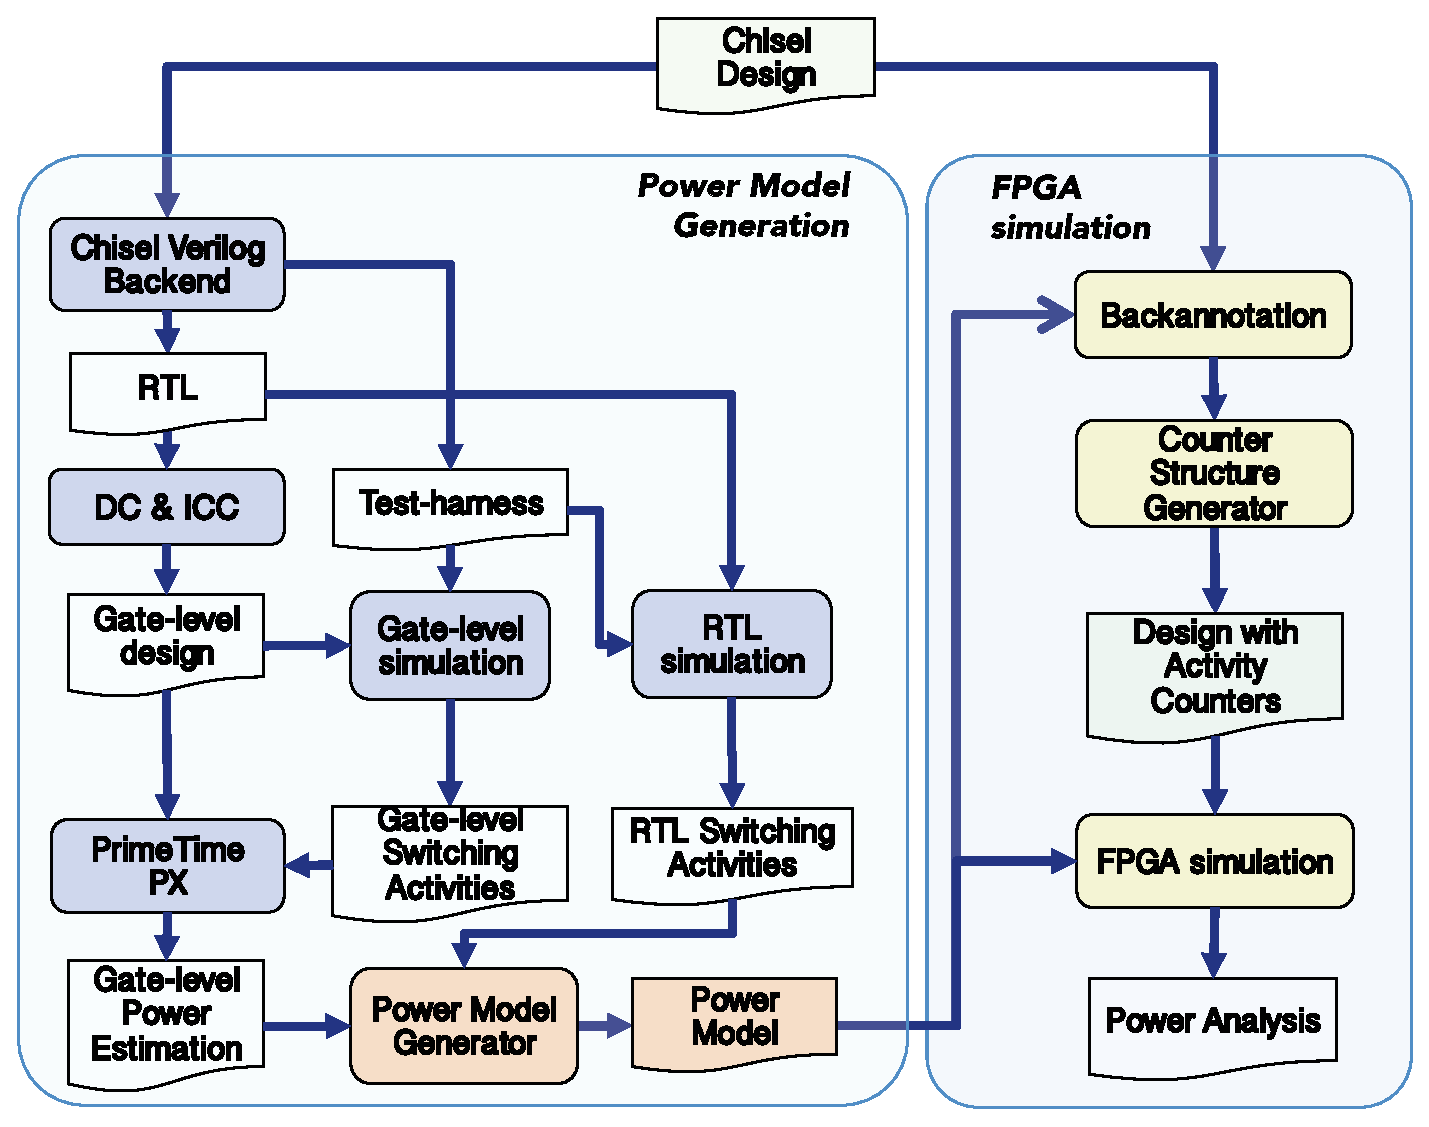
\includegraphics{figure/toolflow}}
  \caption{Tool flow for FPGA-accelerated power simulation}
  \label{fig:toolflow}
\end{figure*}

\section {Tool Flow}
Fig. \ref{fig:toolflow} shows the entire flow for FPGA-accelerated power simulation consisting of two major paths.
We assume that both paths start from the Chisel design.

The left-hand side path is to automatically generate the power models for the target design.
Basically, the power model generator not only approximates the gate-level power estimation with the RTL switching activities,
but also selects the significant RTL signals in the power analysis.

The chisel design is compiled to the RTL design by the Chisel verilog backend,
and to the the gate-level design by the design compiler and the IC compiler.
PrimeTime PX estimates the gate-level power consumption using the gate-level design and its switching activities from gate-level simulation.
In addition, RTL simulation provides the RTL switching activities.
The gate-level power numbers and the RTL switching activities are the inputs for the power model generator.

The power model generator provides the design's linear power model.
It finds the linear relationship between the RTL switching activities and the power consumption of the target design.
To make power measuring tractable, the power generator has to pick the dominant signals in the power model.
The way the power model generator works is explained in Section \ref{sec:main} in detail.

The right-hand side path is to automatically generate the counter structure for FPGA simulation.
FPGA simulation should provide the selected signal activities to calculate the design's power consumption using the power model.
Thus, the Chisel backend backannotates the selected signals from the power model, and generates the activity counter structure.
The design with the activity counters is ported to FPGA, and then FPGA simulation provides the signals' activities from the counter structure.
This enables the detailed power analysis for the target design with its various applications.
\section{Power Model Generator}
\label{sec:main}
\subsection{Linear Power Model}

To obtain power numbers from FPGA simulation, power model generator provides the linear power model of the target design.
Figure \ref{fig:model} shows the graphical representation of the linear power model.
The power model generator solves the linear equation $y = Ac$, 
where $y = [y_1 \ y_2 \ ... \ y_T]$ is the gate-level power consumption at cycle t
and $A = [x_1 \ x_2 \ ... \ x_T]$ is a transition matrix of the target design.
To solve this equation, we take advantage of linear regression with the LMS algorithm.
The solution $c$ of the system is later multiplied by signal activities for power analysis.

\begin{figure}
  \centering
  \resizebox{0.3\columnwidth}{!}{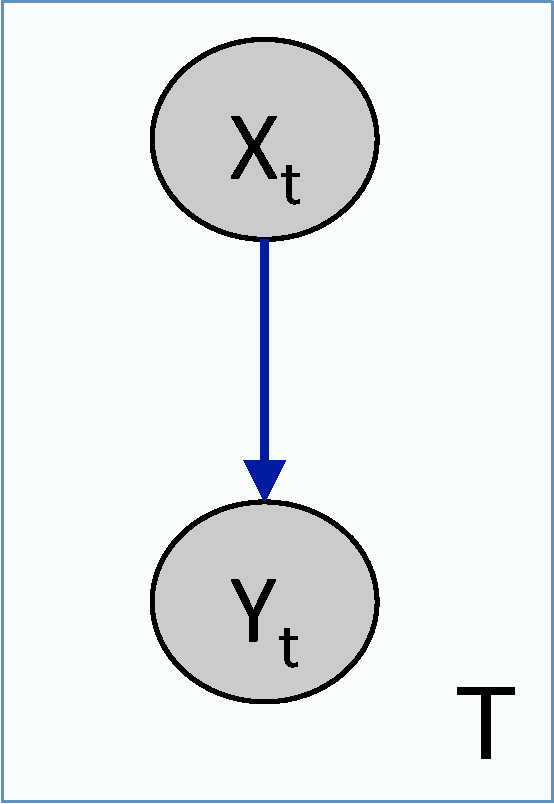
\includegraphics{figure/model}}
  \caption{Graphical representation of the linear power model}
  \label{fig:model}
\end{figure}

In our methodology, the signal activities are provided by FPGA simulation.
Thus, if we have the power model from the target design's microbenchmarks and the signal activities for applications,
we can analyze the power consumption of the specific applications.
Note that FPGA simulation can provide the signal activities much faster than the gate-level simulation or 
cycle-accurate software simulators.

\subsection{LMS Algorithm with Cost Function}

One problem of the linear power model is FPGA simulation cannot provide the switching activities for all the signals.
This is mainly because adding counters for all the signals complicates the original design. 
Thus, we need to pick the signals to be watched during FPGA simulation.

\begin{algorithm}
  \caption{\emph{Take N steps}}
  \begin{algorithmic}[1]
	\STATE Set $f(i) = 0$ and $c^{(0)} = 0$
	\REPEAT
		\STATE Update $f(i) = f(i) + [(c^{(l)})_i * (x_t)_i]$
		\STATE Update $c^{(l+1)} = c^{(l)} + \rho(y_t - c^{(t)T}x_t)$
	\UNTIL{$c^{(l)}$ converges}
  \end{algorithmic}
  \label{alg:lms}
\end{algorithm}

Our approach is to assign cost function to the signals when executing the LMS algorithm.
Algorithm \ref{alg:lms} shows the LMS algorithm with the cost function.

Let $f(i)$ be the cost function for signal $i$. For each iteration of the LMS algorithm,
$f(i)$ is updated according to the current parameter value $c^{(l)}$ and the current i's transition 
in the vector $x_t$. Thus, the cost function means 
the sum of the signal's contribution to each iteration's mean value estimation.
We select the signals with the highest cost function values.


\section{Experiments and results}

\begin{figure*}
	\centering
	\subfloat[Control unit]{
	  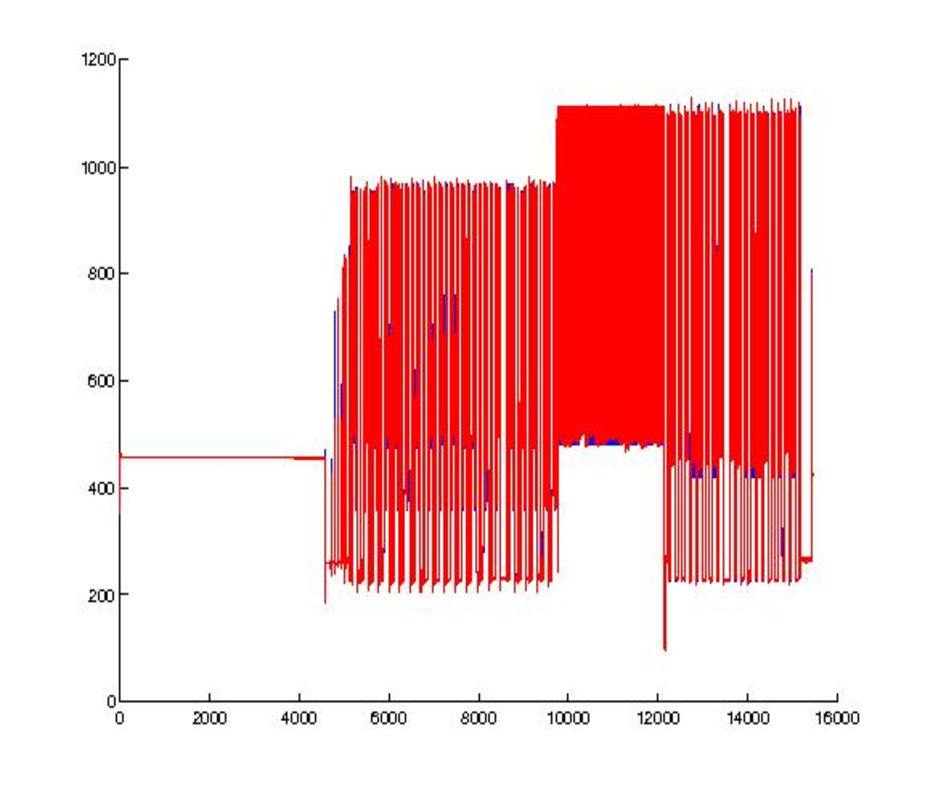
\includegraphics[width=.45\textwidth]{figure/control}
	}
	\subfloat[Data unit]{
	  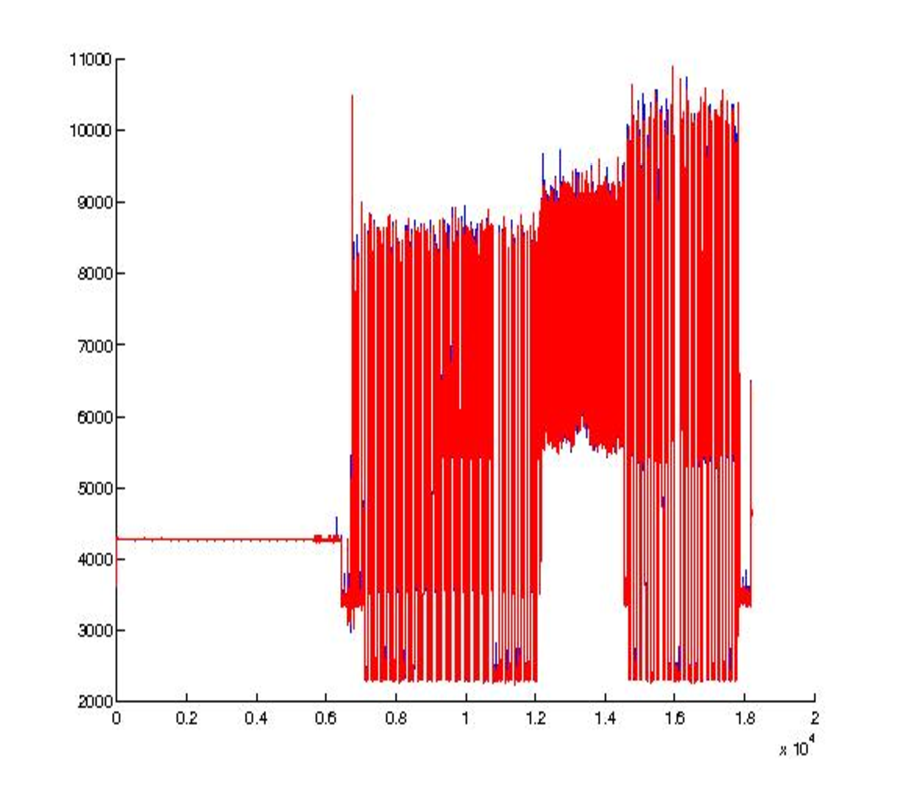
\includegraphics[width=.45\textwidth]{figure/data}
	}
	\\
	\subfloat[Instruction cache]{
	  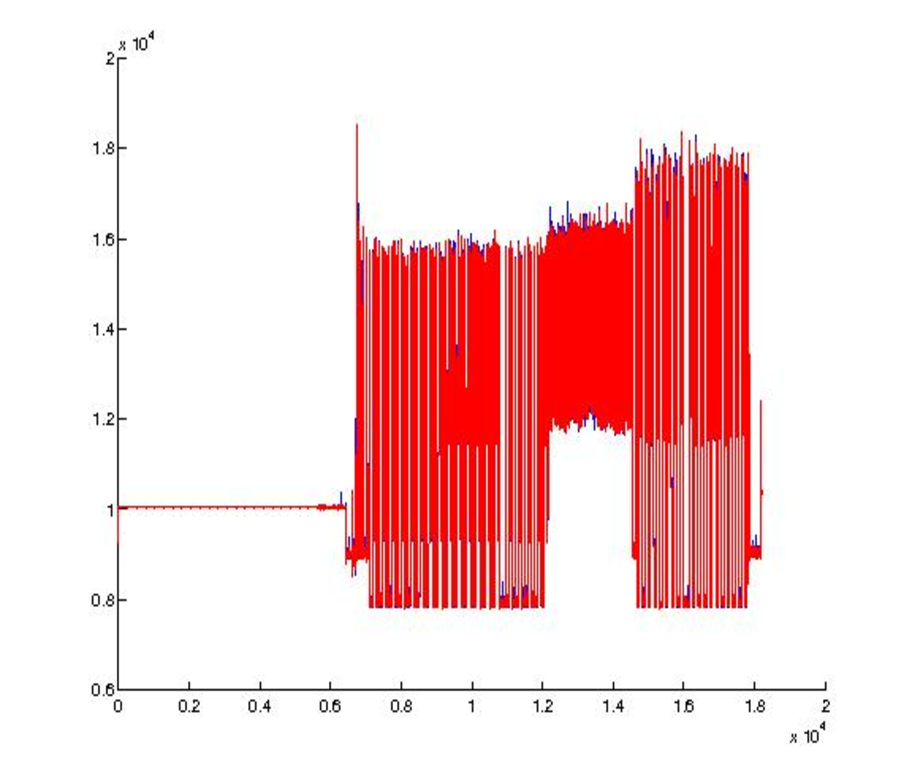
\includegraphics[width=.45\textwidth]{figure/icache}
	}
	\subfloat[Data cache]{
	  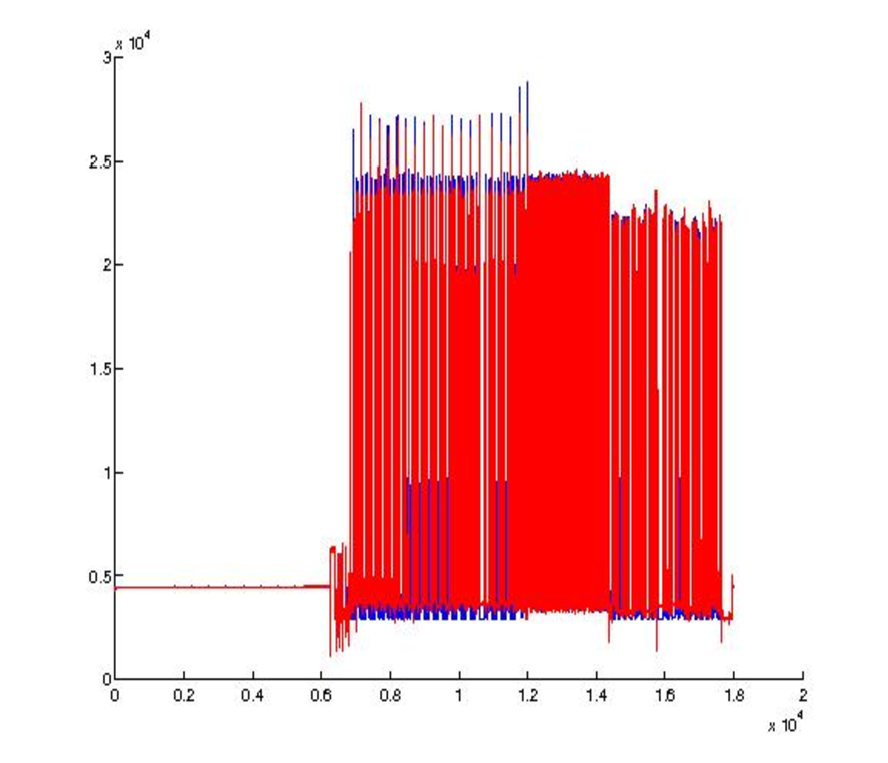
\includegraphics[width=.45\textwidth]{figure/dcache}
	}
	\caption{Comparison between the gate-level power and the linear power model}
	\label{fig:power}
\end{figure*}

Figure \ref{fig:power} shows time-based power analyses for the modules in the RISC-V rocket core.
The red line indicates the gate-level power numbers, and the blue line is the power estimation from the linear power model.
Note that the figures show the linear power model works well for the processors.

\section{Related work}
\label{sec:related_work}

This project is inspired by PrEsto~\cite{PrEsto}, which accelerates power measurement using FPGA. 
It generates linear power models using linear regression, and then the model is mapped onto FPGA. 
However, designers should provide the important signals to the power model generators, and the power calculation logics are hardcoded in FPGA. 
Our approach differs in that the power model generator selects the important signals and we employ a counter-based method to calculate power consumption of the systems.

Bogliolo \textit{et al.}~\cite{Bogliolo2000} suggests regression-based RTL power modeling. 
They exploit linear regression to approximate the design's power consumption with RTL signal activities.
However, this approach cannot be applied to complex designs because it does not reduce the signal list to be watched.
Moreover, it only considers the signals in the border of macro blocks, which attributes to its inaccuracy.

There are several papers about FPGA-accelerated simulations.~\cite{Protoflex,Fast,RAMPGold,FAME,HAsim}
These works show that using FPGAs can reduce the architectural simulation dramatically.
Our project also uses FPGA simulation to accelerated power analysis

Isci \textit{et al.}~\cite{Isci2003} suggests a counter-based method to calculate the system’s power. 
However, it is limited to the real processor, Pentium 4, and thus, not flexible for any other processors. 
Moreover, it has to read the fixed activity counters to calculate power numbers. 
Our approach can be applied to general processor designs and generates activity counters for any important signals.

There are a bunch of attempts to accelerate power measurement of DSP designs~\cite{Coburn2005,Atienza2006,Ghodrat2007}.
However, these are not scalable, so it cannot be applied to complex designs' power measurement.

Bhattacharjee \textit{et al.}~\cite{Bhattacharjee2008} proposed a counter-based method using FPGA emulation. 
This method counts specific events of the processor to calculate power, which requires architectural intuition. 
For this reason, it is not applicable to general logic designs in contrast to our approach.
\section{Conclusion}
In this paper, we propose FPGA-accelerated power simulation with linear power modeling,
which enables fast and accurate power analysis.
The linear power model not only approximates the power consumption with the RTL signal swathing activities,
but reduces the signal set to be watched. 
FPGA simulation make it possible to obtain the selected signal activities quickly.
The power model and the activity counter values from FPGA simulation are used for the detailed power analysis of the target design.

In the future, we will add counters to the target design and evaluate the linear power model with signal activities from FPGA simulation. 
We also plan to model DRAM power with event counters and integrate it with the counter structure to analyze the entire SoC power.

% conference papers do not normally have an appendix

% use section* for acknowledgement
%\section*{Acknowledgment}
%
% trigger a \newpage just before the given reference
% number - used to balance the columns on the last page
% adjust value as needed - may need to be readjusted if
% the document is modified later
%\IEEEtriggeratref{8}
% The "triggered" command can be changed if desired:
%\IEEEtriggercmd{\enlargethispage{-5in}}

% references section

% can use a bibliography generated by BibTeX as a .bbl file
% BibTeX documentation can be easily obtained at:
% http://www.ctan.org/tex-archive/biblio/bibtex/contrib/doc/
% The IEEEtran BibTeX style support page is at:
% http://www.michaelshell.org/tex/ieeetran/bibtex/
\bibliographystyle{IEEEtran}
% argument is your BibTeX string definitions and bibliography database(s)
\bibliography{reference}

%
% <OR> manually copy in the resultant .bbl file
% set second argument of \begin to the number of references
% (used to reserve space for the reference number labels box)
%\begin{thebibliography}{1}

%\bibitem{IEEEhowto:kopka}
%H.~Kopka and P.~W. Daly, \emph{A Guide to \LaTeX}, 3rd~ed.\hskip 1em plus
%  0.5em minus 0.4em\relax Harlow, England: Addison-Wesley, 1999.
%
%\end{thebibliography}




% that's all folks
\end{document}
